
\section{Predictive Tasks on Relational Databases}\label{sec: problem scope}

This section outlines our problem scope: predictive tasks on relational tables. In the process, we define what we mean by relational tables, and how to specify predictive tasks on them. This section focuses exclusively on the structure of data and tasks, laying the groundwork for Section \ref{sec:formal_rl_problem}, which presents our GNN-based modelling approach.


\subsection{Relational Data}
\label{sec:rel_dbs}

\xhdr{A Brief History}
Relational tables and relational databases emerged in the 1970s as a means to standardize data retrieval and management \citep{codd1970relational}. As society digitized, relational databases came to fulfill a foundational purpose, and today are estimated to comprise 72\% of the world's data~\citep{db-engines}. Whilst there is no single agreed upon definition of a relational database, three essential characteristics are shared in all cases (\emph{cf.} Figure \ref{fig: high level outline (fig1)}a):
\begin{enumerate}
    \item Data is stored in multiple tables.
    \item Each row in each table contains an \emph{entity}, which possesses a unique primary key ID, along with multiple attributes stored as columns of the table.
    \item One entity may refer to another entity using a foreign key---the primary key of another entity.
\end{enumerate}

As well as a standardized storage system, relational databases typically come equipped with a powerful set of \emph{relational operations}, which are used to manipulate and access data. \cite{codd1970relational} introduced 8 relational operations, including set operations such as taking the union of two tables, and other operations such as \emph{joining} two tables based on their common attributes. Popular query languages such as SQL \citep{chamberlin1974sequel} provide commercial-grade implementations of a wide variety of relational operations.
Next we formally define relational data, as suits our purposes.


\xhdr{Definition of Relational Databases} A relational database $(\mathcal T, \mathcal L)$ is comprised of a collection of tables $\mathcal T = \{T_1 , \ldots , T_n\}$, and links between tables $\mathcal L \subseteq \mathcal T \times \mathcal T$ (\emph{cf.} Figure \ref{fig: end to end pipeline}a). A link $L = (T_{\rm fkey}$, $T_{\rm pkey})$ between tables exists if a foreign key column in $T_{\rm fkey}$ points to a primary key column of $T_{\rm pkey}$.
Each table is a set $T = \{v_1, ..., v_{n_T}\}$, whose elements $v_i \in T$ are called rows, or entities (\emph{cf.} Figure \ref{fig: end to end pipeline}b). Each entity $v \in T$, has four constituent parts $v = (p_v, \mathcal K_v, x_v, t_v)$: 
\begin{enumerate}
    \item \textbf{Primary key} $p_v$, that uniquely identifies the entity $v$. 
    \item \textbf{Foreign keys} $\mathcal K_v\subseteq \{p_{v'}:  v' \in T'\text{ and } (T, T') \in \mathcal L \}$, defining links between element $v\in T$ to elements $v' \in T'$, where $p_{v'}$ is the primary key of an entity $v'$ in table $T'$. 
    \item \textbf{Attributes} $x_v$, holding the informational content of the entity. % \matthias{can we define $d_T$?}
    \item \textbf{Timestamp} An optional timestamp $t_v$, indicating the time an event occurred. 
\end{enumerate}

For example, the \tbl{Transactions} table in Figure \ref{fig: end to end pipeline}a has the primary key (\tbl{TransactionID}), two foreign keys (\tbl{ProductID} and \tbl{CustomerID}), one attribute (\tbl{Price}), and timestamp column (\tbl{Timestamp}). Similarly, the \tbl{Products} table has the primary key (\tbl{ProductID}), no foreign keys, attributes (\tbl{Description}, \tbl{Image} and \tbl{Size}), and no timestamp. The connection between foreign keys and primary keys is illustrated by black connecting lines in Figure \ref{fig: end to end pipeline}.

In general, the attributes in table $T$ contain $d_T$ values: $x_v= (x_v^1, \ldots , x_v^{d_T})$, each belonging to a particular column. Critically, all entities in the same table have the same columns (values may be absent). Formally, this is described by membership  $x_v= (x_v^1, \ldots , x_v^{d_T}) \in \mathcal A_T^1 \times \ldots \times \mathcal A_T^{d_T}$, where $\mathcal A^i_T$ denotes the value space of $i$-th column of table $T$, and is shared between all entities $v \in T$.
%(such as numerical value, categorical value, image, or text spaces)
For example, the \tbl{Products} table from Fig.~\ref{fig: end to end pipeline}a contains three different attributes: the \emph{product description} (text type), the \emph{image} of the product (image type), and the \emph{size} of the product (numerical type). Each of these types has their own encoders as discussed in Sec.~\ref{sec:encoders}. 


\xhdr{Fact and Dimension Tables} Tables are categorized into two types, \emph{fact} or \emph{dimension},  with complementary roles \citep{ullman-book}. Dimension tables provide contextual information, such as biographical information, macro statistics (such as number of beds in a hospital), or immutable properties, such as the size of a product (as in the \tbl{Products} table in Figure \ref{fig: end to end pipeline}a). Dimension tables tend to have relatively few rows, as it is limited to one per real-world object. Fact tables record interactions between other entities, such as all patient admissions to hospital, or all customer transactions (as in the \tbl{Transactions} table in Figure \ref{fig: end to end pipeline}a). Since entities can interact repeatedly, fact tables often contain the majority of rows in a relational database. Typically, features in dimension tables are static over their whole lifetime, while fact tables usually contain temporal information with a dedicated time column that denotes the time of appearance.

\xhdr{Temporality as a First-Class Citizen}

Relational data evolves over time as events occur and are recorded. 
%
This is captured by the (optional) timestamp $t_v$ attached to each entity $v$. For example, each transaction in \tbl{Transactions} has a time stamp.
Furthermore, many \emph{tasks} of interest involve forecasting future events. For example, how much will a customer spend in next $k$ days. It is therefore essential that time is conferred a special status unlike other attributes.  Our formulation, introduced in Section \ref{sec:formal_rl_problem}, achieves this through a temporal message passing scheme (similar to \cite{rossi2020temporal}), that only permits nodes to receive messages from neighbors with earlier timestamps. This ensures that models do not leak information from the future during training, avoiding shortcut decision rules that achieve high training accuracy but fail at test time \citep{geirhos2020shortcut}. It also means that model-extracted features are automatically updated as new relational data is added.

\subsection{From Task to Training Table}
\label{sec:predictive_labels}

There are many practically interesting machine learning tasks defined over relational databases, such as predicting the response of a patient to treatment, or the future sales of a product.
These tasks involve predicting the future state of the entities of interest.
Given a task we wish to solve, how can we create \emph{ground truth labels} to supervise machine learning models training? 

Our key insight is that we can generate training labels using historical data.
For instance, at time $t$, ground truth labels for predicting ``how much each customer will buy in the next $90$ days?'' are computed by summing up each customer's spending within the interval $t$ and $t+90$ days. Importantly, as long as $t+90$ is less than the most recent timestamp in the database, then these ground truth labels can be computed \emph{purely from historical data} without any need for external annotation. Further, by choosing different time points $t$ across the database time horizon, it is possible to naturally compute many ground truth training labels for each entity.

To hold the labels for a new predictive task, we introduce a new table known as a \emph{training table} $T_\text{train}$ (Fig.~\ref{fig:training_table}).
 Each entity $v=(\mathcal K_v,t_v,y_v)$ in the training table $T_\text{train}$ has three components: (1) A (set of) foreign keys $\mathcal K_v$ indicating the entities the training example is associated to, (2) a timestamp $t_v$, and (3) the ground truth label itself $y_v$.  In contrast to tabular learning settings, the training table does \emph{not} contain input data $x_v$. The training table is linked to the main relational database $(\mathcal T, \mathcal L)$ by updating: (1)  the set of tables to $\mathcal T  \cup \{{T_\text{train}}\}$, and (2) the links between tables to $ \mathcal L \cup \mathcal{L}_{T_\text{train}}$, where $\mathcal{L}_{T_\text{train}}$ specifies tables that training table keys $\mathcal K_v$ point to. 
 
 
As discussed in Sec. \ref{sec:rel_dbs}, careful handling of what data the model sees during training is crucial in order to ensure temporal leakage does not happen. This is achieved using the training timestamp. When the model is trained to output target $y_v$ for entity $v$ with timestamp $t_v$, temporal consistency is ensured by only permitting the model to receive input information from entities $u$ with timestamp $t_u \leq t_v$ (see Sec. \ref{sec:temporal_sampling} for details on training sampling). 
 

\begin{figure}[t] % 'h' for here
  \centering
    \begin{tikzpicture}

\node (ex1) at (5,0)
{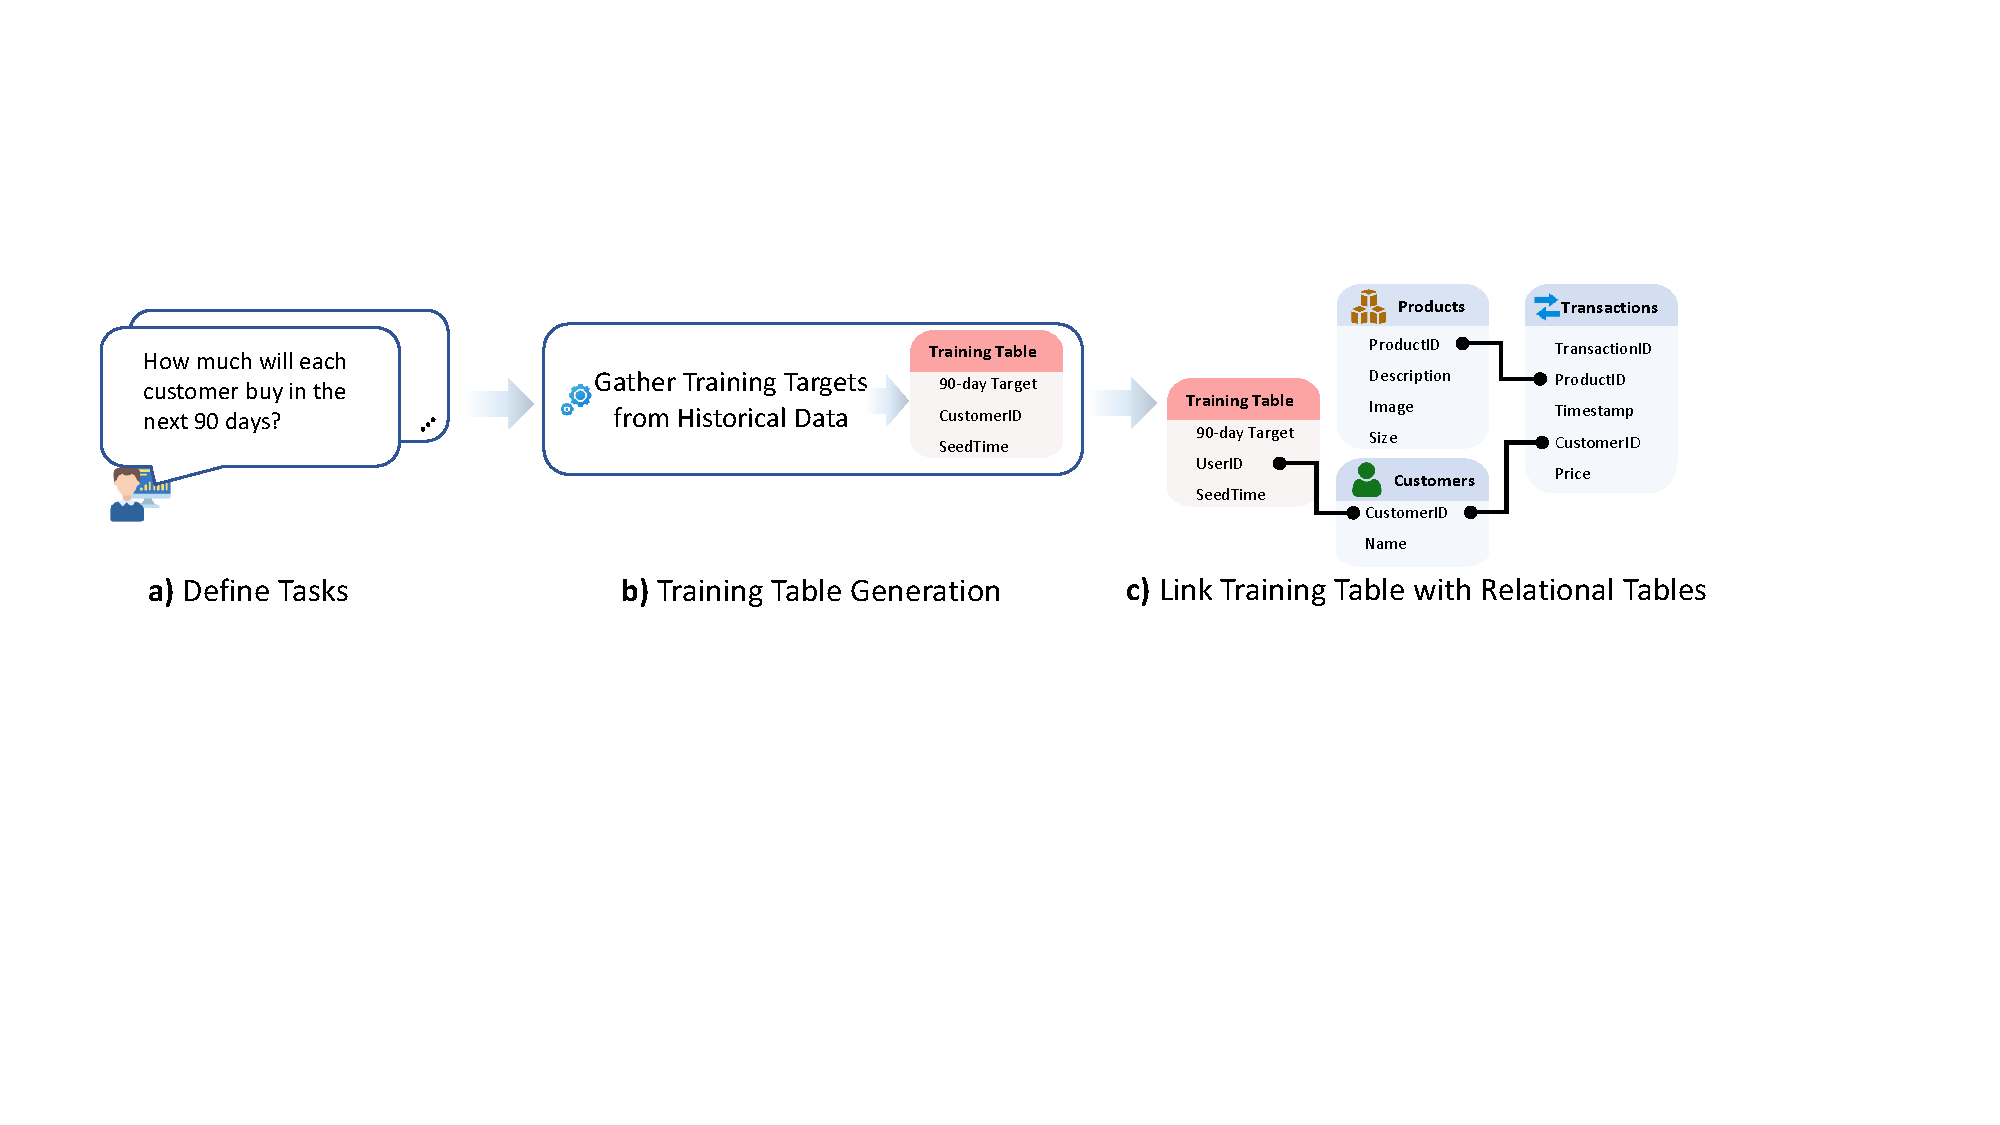
\includegraphics[trim={0.2cm 0.8cm 0cm 0cm}, clip, scale=0.52]{figs/f2.pdf}};
\node[scale=0.8] at (-0.5,-1.5) { \textbf{(a)} Define Tasks};

\node[scale=0.8] at (4,-1.51) { \textbf{(b)} Training Table Generation};

\node[scale=0.8] at (9.4,-1.5) { \textbf{(c)} Link to Relational Tables};


\end{tikzpicture}\vspace{-0.4cm}
  \caption{\textbf{Predictive Task Definition.} A task over relational data is defined by attaching an additional \emph{training table} to the existing linked tables. A training table entity specifies \textbf{(a)} ground truth label computed from historical information \textbf{(b)} the entity ID(s) the labels correspond to, and \textbf{(c)} a timestamp that controls what data the model can use to predict this label.}
  \label{fig:training_table}
\end{figure}


Thus, the purpose of the training table is twofold: to specify training \emph{inputs} and \emph{outputs} of the machine learning model. First, it provides supervision on the model \emph{output} by specifying the the entities and their target training labels. Second, in the case of temporal tasks, the training table specifies the model \emph{input} by specifying the timestamp at which each historical training label is generated. 



This training table formulation can model a wide range of predictive tasks on relational databases:
\begin{itemize}
    \item {\bf Node-level prediction tasks} (\eg, multi-class classification, multi-label classification, regression): The training table has three columns \tbl{(EntityID, Label, Time)}, indicating the foreign key, target label, and timestamp columns, respectively.
    \item {\bf Link prediction tasks}: The training table has columns \tbl{(SourceEntityID, TargetEntityID, Label, Time)}, indicating the foreign key columns for the source/target nodes, and the target label, and timestamp, respectively.
    \item \textbf{Temporal and static prediction tasks}: Temporal tasks make predictions about the future (and require a seed time), while non-temporal tasks impute missing values (\tbl{Time} is dropped).
\end{itemize}



\xhdr{Training Table Generation} In practice, training tables can be computed using time-conditioned SQL queries from historic data in the database. Given a query that describes the prediction targets for all prediction entities, e.g. the sum of sells grouped by products, from time $t$ to time $t+\delta$ in the future, we can move $t$ back in time in fixed intervals to gather historical training, validation and test targets for all entities (\emph{cf.} Fig.~\ref{fig:training_table}b). We store $t$ as timestamp for the targets gathered in each step.

